\documentclass[]{elsarticle} %review=doublespace preprint=single 5p=2 column
%%% Begin My package additions %%%%%%%%%%%%%%%%%%%
\usepackage[hyphens]{url}

\usepackage{lineno} % add
\providecommand{\tightlist}{%
  \setlength{\itemsep}{0pt}\setlength{\parskip}{0pt}}

\usepackage{graphicx}
%%%%%%%%%%%%%%%% end my additions to header

\usepackage[T1]{fontenc}
\usepackage{lmodern}
\usepackage{amssymb,amsmath}
\usepackage{ifxetex,ifluatex}
\usepackage{fixltx2e} % provides \textsubscript
% use upquote if available, for straight quotes in verbatim environments
\IfFileExists{upquote.sty}{\usepackage{upquote}}{}
\ifnum 0\ifxetex 1\fi\ifluatex 1\fi=0 % if pdftex
  \usepackage[utf8]{inputenc}
\else % if luatex or xelatex
  \usepackage{fontspec}
  \ifxetex
    \usepackage{xltxtra,xunicode}
  \fi
  \defaultfontfeatures{Mapping=tex-text,Scale=MatchLowercase}
  \newcommand{\euro}{€}
\fi
% use microtype if available
\IfFileExists{microtype.sty}{\usepackage{microtype}}{}
\usepackage[left=3cm,right=3cm,top=3cm,bottom=3cm]{geometry}
\bibliographystyle{elsarticle-harv}
\usepackage{color}
\usepackage{fancyvrb}
\newcommand{\VerbBar}{|}
\newcommand{\VERB}{\Verb[commandchars=\\\{\}]}
\DefineVerbatimEnvironment{Highlighting}{Verbatim}{commandchars=\\\{\}}
% Add ',fontsize=\small' for more characters per line
\newenvironment{Shaded}{}{}
\newcommand{\AlertTok}[1]{\textcolor[rgb]{1.00,0.00,0.00}{#1}}
\newcommand{\AnnotationTok}[1]{\textcolor[rgb]{0.00,0.50,0.00}{#1}}
\newcommand{\AttributeTok}[1]{#1}
\newcommand{\BaseNTok}[1]{#1}
\newcommand{\BuiltInTok}[1]{#1}
\newcommand{\CharTok}[1]{\textcolor[rgb]{0.00,0.50,0.50}{#1}}
\newcommand{\CommentTok}[1]{\textcolor[rgb]{0.00,0.50,0.00}{#1}}
\newcommand{\CommentVarTok}[1]{\textcolor[rgb]{0.00,0.50,0.00}{#1}}
\newcommand{\ConstantTok}[1]{#1}
\newcommand{\ControlFlowTok}[1]{\textcolor[rgb]{0.00,0.00,1.00}{#1}}
\newcommand{\DataTypeTok}[1]{#1}
\newcommand{\DecValTok}[1]{#1}
\newcommand{\DocumentationTok}[1]{\textcolor[rgb]{0.00,0.50,0.00}{#1}}
\newcommand{\ErrorTok}[1]{\textcolor[rgb]{1.00,0.00,0.00}{\textbf{#1}}}
\newcommand{\ExtensionTok}[1]{#1}
\newcommand{\FloatTok}[1]{#1}
\newcommand{\FunctionTok}[1]{#1}
\newcommand{\ImportTok}[1]{#1}
\newcommand{\InformationTok}[1]{\textcolor[rgb]{0.00,0.50,0.00}{#1}}
\newcommand{\KeywordTok}[1]{\textcolor[rgb]{0.00,0.00,1.00}{#1}}
\newcommand{\NormalTok}[1]{#1}
\newcommand{\OperatorTok}[1]{#1}
\newcommand{\OtherTok}[1]{\textcolor[rgb]{1.00,0.25,0.00}{#1}}
\newcommand{\PreprocessorTok}[1]{\textcolor[rgb]{1.00,0.25,0.00}{#1}}
\newcommand{\RegionMarkerTok}[1]{#1}
\newcommand{\SpecialCharTok}[1]{\textcolor[rgb]{0.00,0.50,0.50}{#1}}
\newcommand{\SpecialStringTok}[1]{\textcolor[rgb]{0.00,0.50,0.50}{#1}}
\newcommand{\StringTok}[1]{\textcolor[rgb]{0.00,0.50,0.50}{#1}}
\newcommand{\VariableTok}[1]{#1}
\newcommand{\VerbatimStringTok}[1]{\textcolor[rgb]{0.00,0.50,0.50}{#1}}
\newcommand{\WarningTok}[1]{\textcolor[rgb]{0.00,0.50,0.00}{\textbf{#1}}}
\usepackage{longtable,booktabs,array}
\usepackage{calc} % for calculating minipage widths
% Correct order of tables after \paragraph or \subparagraph
\usepackage{etoolbox}
\makeatletter
\patchcmd\longtable{\par}{\if@noskipsec\mbox{}\fi\par}{}{}
\makeatother
% Allow footnotes in longtable head/foot
\IfFileExists{footnotehyper.sty}{\usepackage{footnotehyper}}{\usepackage{footnote}}
\makesavenoteenv{longtable}
\ifxetex
  \usepackage[setpagesize=false, % page size defined by xetex
              unicode=false, % unicode breaks when used with xetex
              xetex]{hyperref}
\else
  \usepackage[unicode=true]{hyperref}
\fi
\hypersetup{breaklinks=true,
            bookmarks=true,
            pdfauthor={},
            pdftitle={Livin' on the edge: Precision yield data shows evidence of ecosystem services from field boundaries},
            colorlinks=false,
            urlcolor=blue,
            linkcolor=magenta,
            pdfborder={0 0 0}}
\urlstyle{same}  % don't use monospace font for urls

\setcounter{secnumdepth}{5}
% Pandoc toggle for numbering sections (defaults to be off)

% Pandoc citation processing
\newlength{\cslhangindent}
\setlength{\cslhangindent}{1.5em}
\newlength{\csllabelwidth}
\setlength{\csllabelwidth}{3em}
% for Pandoc 2.8 to 2.10.1
\newenvironment{cslreferences}%
  {}%
  {\par}
% For Pandoc 2.11+
\newenvironment{CSLReferences}[2] % #1 hanging-ident, #2 entry spacing
 {% don't indent paragraphs
  \setlength{\parindent}{0pt}
  % turn on hanging indent if param 1 is 1
  \ifodd #1 \everypar{\setlength{\hangindent}{\cslhangindent}}\ignorespaces\fi
  % set entry spacing
  \ifnum #2 > 0
  \setlength{\parskip}{#2\baselineskip}
  \fi
 }%
 {}
\usepackage{calc}
\newcommand{\CSLBlock}[1]{#1\hfill\break}
\newcommand{\CSLLeftMargin}[1]{\parbox[t]{\csllabelwidth}{#1}}
\newcommand{\CSLRightInline}[1]{\parbox[t]{\linewidth - \csllabelwidth}{#1}\break}
\newcommand{\CSLIndent}[1]{\hspace{\cslhangindent}#1}

% Pandoc header
\makeatletter \def\ps@pprintTitle{  \let\@oddhead\@empty  \let\@evenhead\@empty  \def\@oddfoot{\centerline{\thepage}} \let\@evenfoot\@oddfoot} \makeatother \usepackage{float} \floatplacement{figure}{H} \newcommand{\beginsupplement}{\setcounter{table}{0} \renewcommand{\thetable}{S\arabic{table}} \setcounter{figure}{0} \renewcommand{\thefigure}{S\arabic{figure}}} 
\usepackage{booktabs}
\usepackage{longtable}
\usepackage{array}
\usepackage{multirow}
\usepackage{wrapfig}
\usepackage{float}
\usepackage{colortbl}
\usepackage{pdflscape}
\usepackage{tabu}
\usepackage{threeparttable}
\usepackage{threeparttablex}
\usepackage[normalem]{ulem}
\usepackage{makecell}
\usepackage{xcolor}

\begin{document}

\hypertarget{appendix-a-supplemental-information}{%
\section*{Appendix A: Supplemental Information}\label{appendix-a-supplemental-information}}
\addcontentsline{toc}{section}{Appendix A: Supplemental Information}

\setcounter{table}{0} \renewcommand{\thetable}{S\arabic{table}} \setcounter{figure}{0} \renewcommand{\thefigure}{S\arabic{figure}}

\begin{figure}
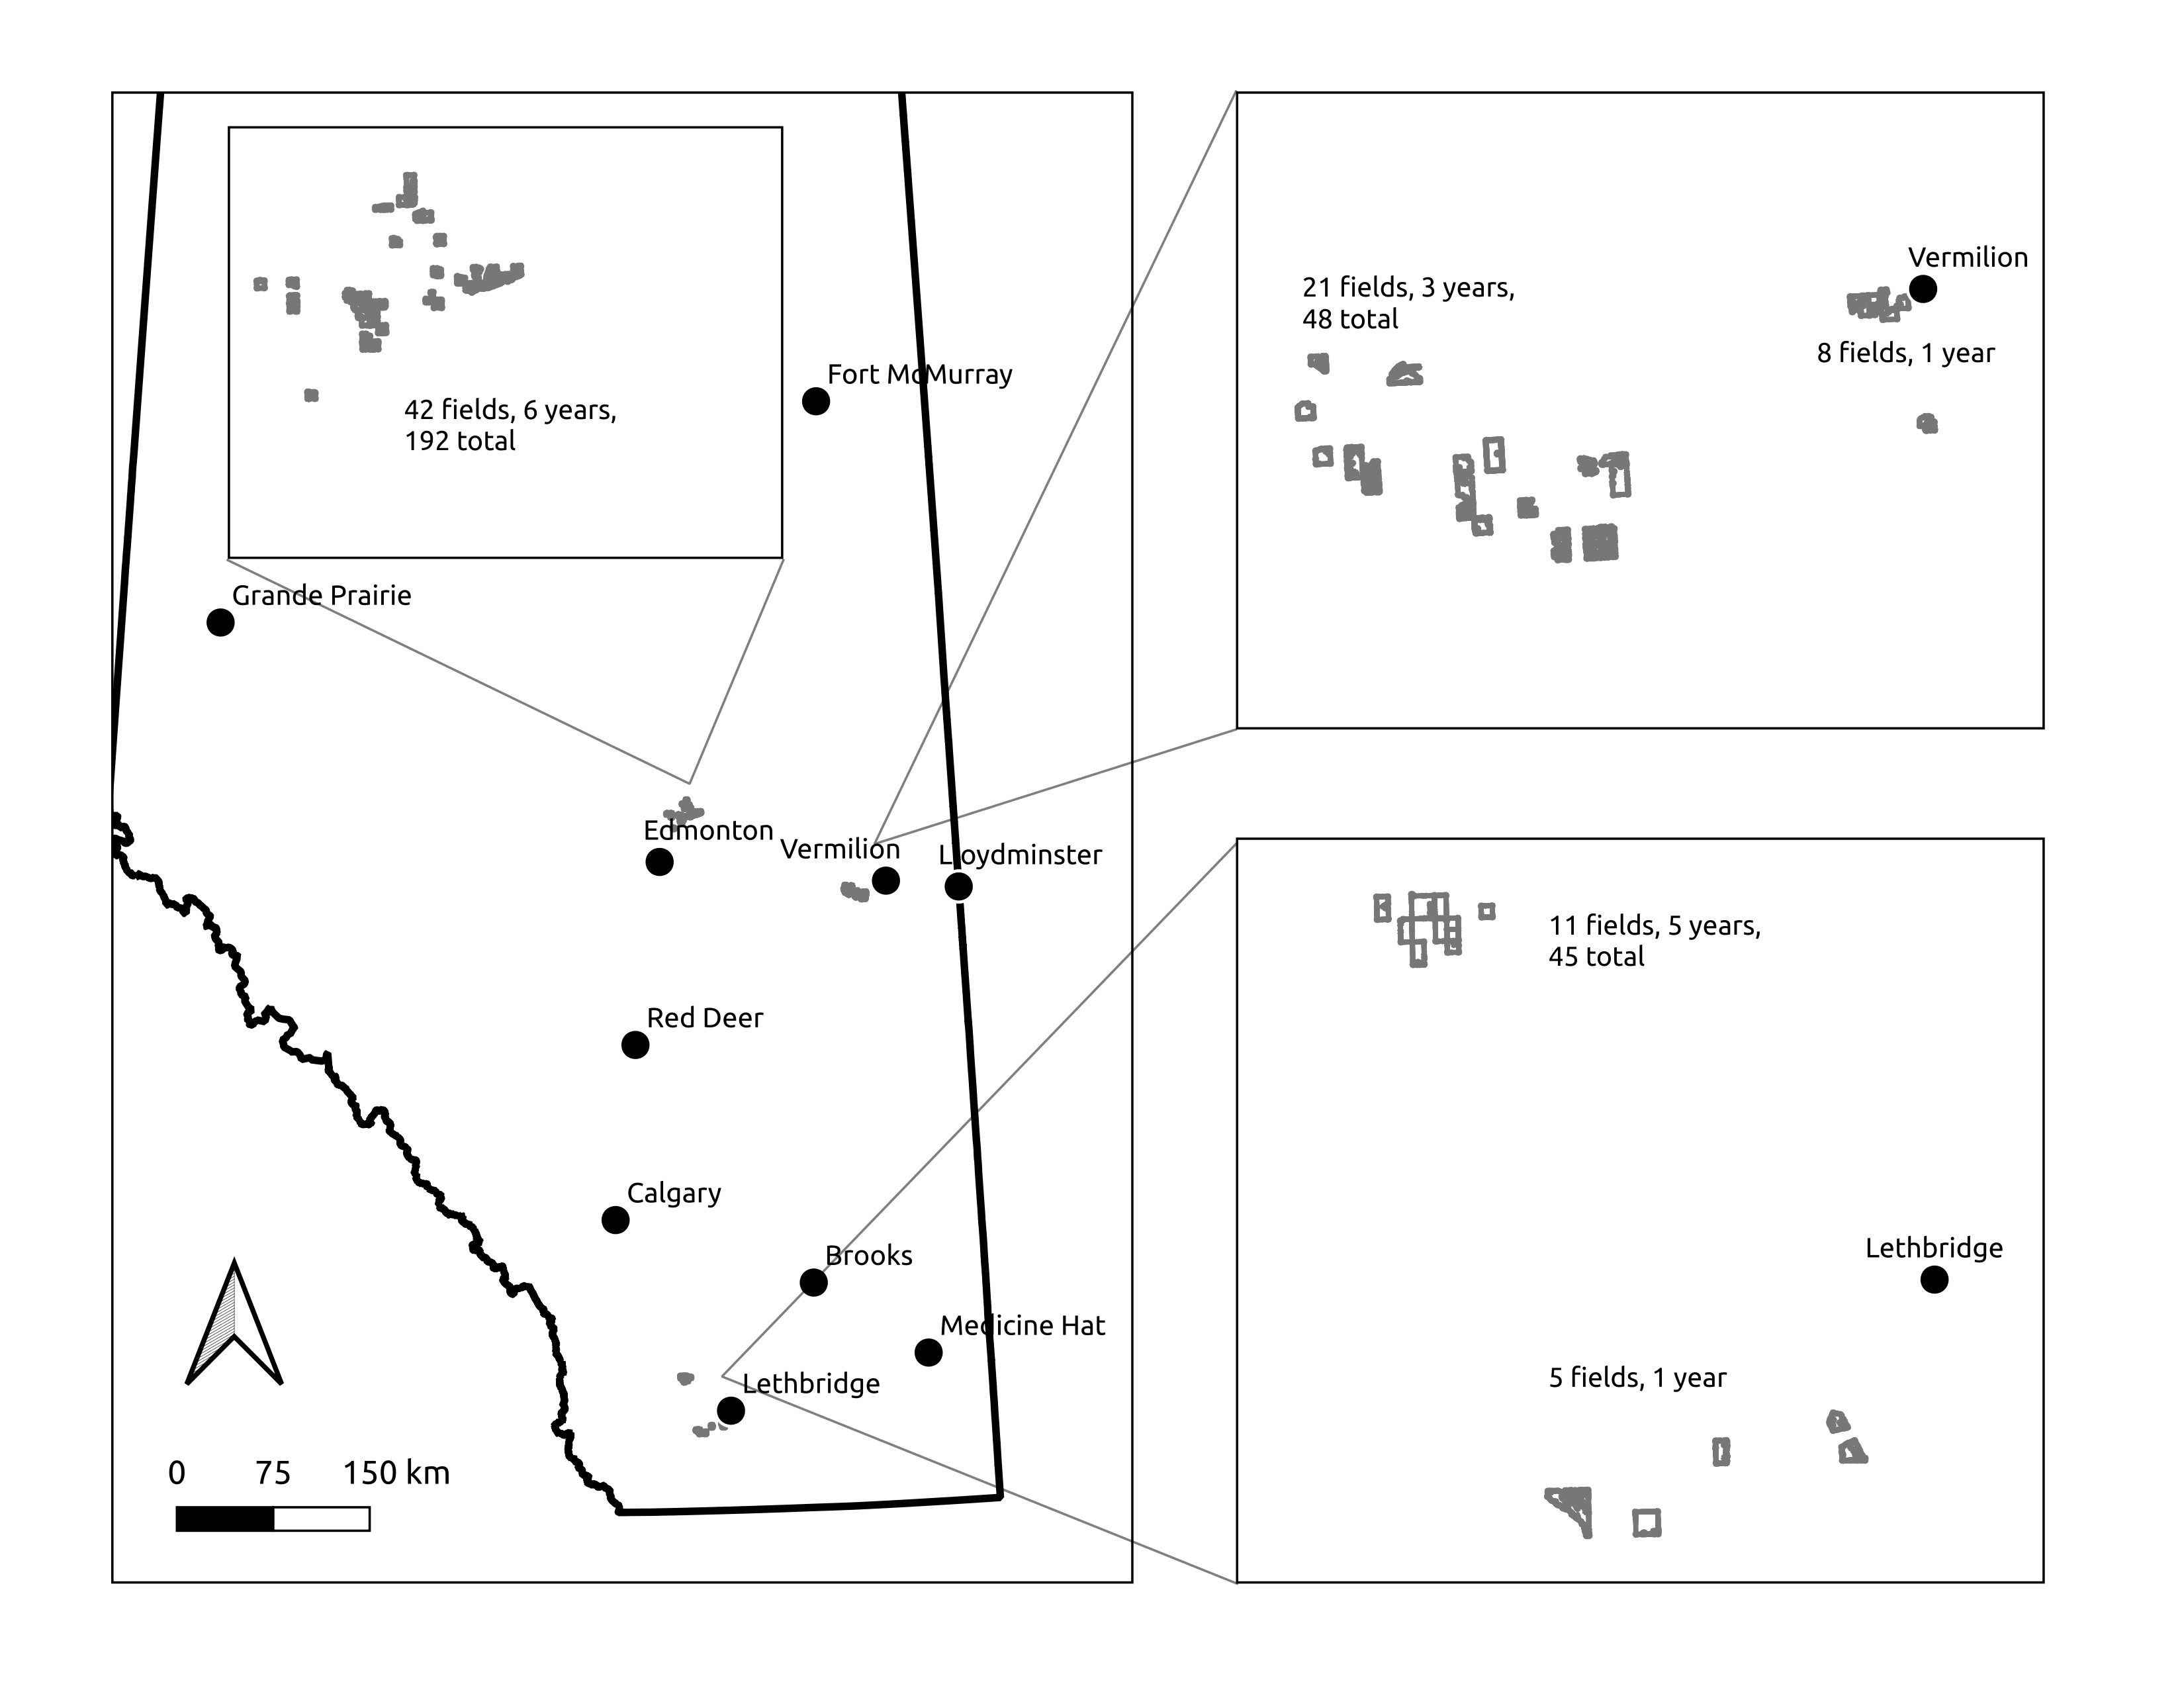
\includegraphics[width=1\linewidth]{Field Locations} \caption{Locations of fields that data were collected from.}
\end{figure}

\begin{figure}
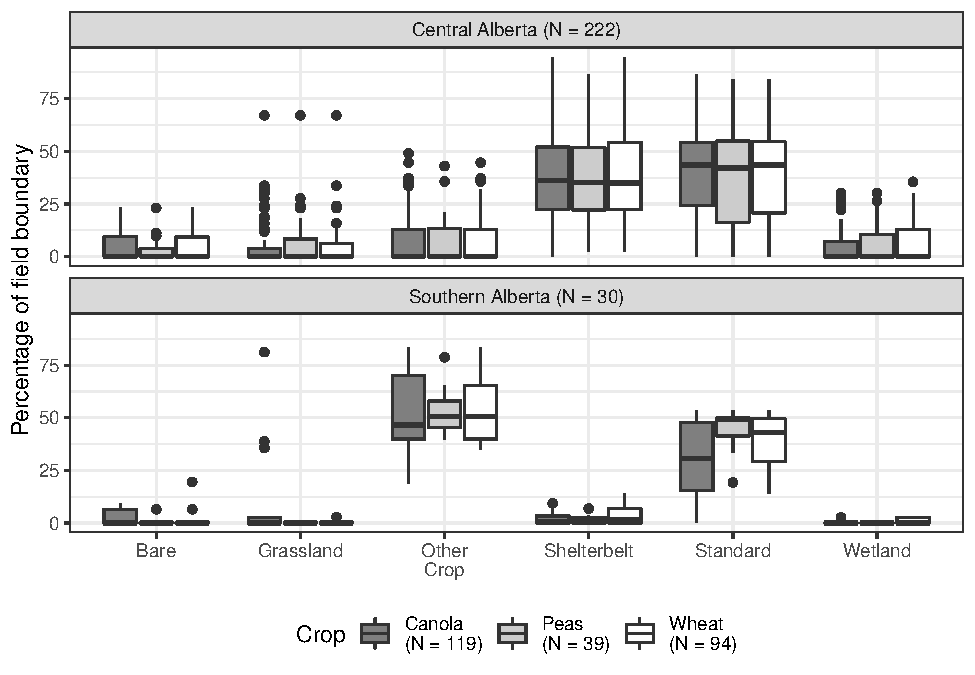
\includegraphics[width=1\linewidth]{boundaryTypes-1} \caption{Boxplot of field boundary compositions across sampled fields. The x-axis indicates the boundary type, while the y-axis indicates the percentage of all field boundaries covered by that boundary type.}
\end{figure}

\newpage

\hypertarget{appendix-b-r-code-for-data-filtering}{%
\section*{Appendix B: R Code for Data Filtering}\label{appendix-b-r-code-for-data-filtering}}
\addcontentsline{toc}{section}{Appendix B: R Code for Data Filtering}

\begin{Shaded}
\begin{Highlighting}[]
\CommentTok{\# Helper functions {-}{-}{-}{-}{-}{-}{-}{-}{-}{-}{-}{-}{-}{-}{-}{-}{-}}

\CommentTok{\#"Inlier" spatial filtering procedure from Vega et al 2019, rewritten to work}
\CommentTok{\#with sf + dplyr. Returns boolean}
\NormalTok{vegaFilter }\OtherTok{\textless{}{-}} \ControlFlowTok{function}\NormalTok{(data,ycol,}\AttributeTok{pvalCutoff=}\FloatTok{0.05}\NormalTok{,}\AttributeTok{nDist=}\DecValTok{40}\NormalTok{)\{}
  \FunctionTok{require}\NormalTok{(sf)}
  \FunctionTok{require}\NormalTok{(sp)}
  \FunctionTok{require}\NormalTok{(spdep)}
  \FunctionTok{require}\NormalTok{(tidyverse)}
  
  \ControlFlowTok{if}\NormalTok{(}\SpecialCharTok{!}\FunctionTok{any}\NormalTok{(}\FunctionTok{class}\NormalTok{(data) }\SpecialCharTok{\%in\%} \StringTok{\textquotesingle{}sf\textquotesingle{}}\NormalTok{)) }\FunctionTok{stop}\NormalTok{(}\StringTok{\textquotesingle{}Dataframe must be sf object\textquotesingle{}}\NormalTok{)}
  
\NormalTok{  coords }\OtherTok{\textless{}{-}} \FunctionTok{st\_coordinates}\NormalTok{(data) }\CommentTok{\#Get coordinates in matrix form}
  
  \CommentTok{\#Get neighbourhood weights from 0 to ndist meters}
\NormalTok{  nWeights }\OtherTok{\textless{}{-}} \FunctionTok{dnearneigh}\NormalTok{(coords,}\DecValTok{0}\NormalTok{,nDist) }
  
  \ControlFlowTok{if}\NormalTok{(}\FunctionTok{any}\NormalTok{(}\FunctionTok{sapply}\NormalTok{(nWeights,length)}\SpecialCharTok{==}\DecValTok{1}\NormalTok{))\{}
    \FunctionTok{warning}\NormalTok{(}\StringTok{\textquotesingle{}Some points had no neighbours and were removed\textquotesingle{}}\NormalTok{)}
\NormalTok{  \} }
  
  \CommentTok{\#Get neighbourhood indices for each point (which other points are in this}
  \CommentTok{\#point\textquotesingle{}s neighbourhood?)}
\NormalTok{  nIndices }\OtherTok{\textless{}{-}} \FunctionTok{nb2listw}\NormalTok{(nWeights, }\AttributeTok{style =} \StringTok{"W"}\NormalTok{,}\AttributeTok{zero.policy =} \ConstantTok{TRUE}\NormalTok{) }
  
\NormalTok{  yield }\OtherTok{\textless{}{-}} \FunctionTok{pull}\NormalTok{(data,\{\{ycol\}\}) }\CommentTok{\#Get yield data column}
  
  \CommentTok{\#Local Moran\textquotesingle{}s I for each neighbourhood}
\NormalTok{  LM }\OtherTok{\textless{}{-}} \FunctionTok{localmoran}\NormalTok{(yield,nIndices,}\AttributeTok{p.adjust.method=}\StringTok{"bonferroni"}\NormalTok{,}
                   \AttributeTok{alternative =}\StringTok{"less"}\NormalTok{)}
  
\NormalTok{  results }\OtherTok{\textless{}{-}} \FunctionTok{data.frame}\NormalTok{(LM) }\SpecialCharTok{\%\textgreater{}\%} 
    \FunctionTok{rename}\NormalTok{(}\StringTok{\textquotesingle{}pval\textquotesingle{}}\OtherTok{=}\FunctionTok{contains}\NormalTok{(}\StringTok{\textquotesingle{}Pr.z.\textquotesingle{}}\NormalTok{)) }\SpecialCharTok{\%\textgreater{}\%} 
    \CommentTok{\#Filter negative Ii and pvals \textless{} 0.05}
    \FunctionTok{mutate}\NormalTok{(}\AttributeTok{keepThese=}\NormalTok{ Ii }\SpecialCharTok{\textgreater{}} \DecValTok{0} \SpecialCharTok{|}\NormalTok{ pval }\SpecialCharTok{\textgreater{}}\NormalTok{ pvalCutoff) }\SpecialCharTok{\%\textgreater{}\%} 
    \CommentTok{\#NAs (points had no neighbours)}
    \FunctionTok{mutate}\NormalTok{(}\AttributeTok{keepThese=}\FunctionTok{ifelse}\NormalTok{(}\FunctionTok{is.na}\NormalTok{(keepThese),}\ConstantTok{FALSE}\NormalTok{,keepThese)) }
  
\NormalTok{  ret }\OtherTok{\textless{}{-}} \FunctionTok{pull}\NormalTok{(results)}
  \FunctionTok{return}\NormalTok{(ret)}
\NormalTok{\}}

\CommentTok{\#Function to filter anything above a certain z{-}score. Returns boolean}
\NormalTok{ZscoreFilter }\OtherTok{\textless{}{-}} \ControlFlowTok{function}\NormalTok{(x,}\AttributeTok{z=}\DecValTok{3}\NormalTok{)\{}
\NormalTok{  xmean }\OtherTok{\textless{}{-}} \FunctionTok{mean}\NormalTok{(x,}\AttributeTok{na.rm=}\ConstantTok{TRUE}\NormalTok{)}
\NormalTok{  xsd }\OtherTok{\textless{}{-}} \FunctionTok{sd}\NormalTok{(x,}\AttributeTok{na.rm=}\ConstantTok{TRUE}\NormalTok{)}
\NormalTok{  zscore }\OtherTok{\textless{}{-}} \FunctionTok{abs}\NormalTok{(((x}\SpecialCharTok{{-}}\NormalTok{xmean)}\SpecialCharTok{/}\NormalTok{xsd))}
\NormalTok{  zscore}\SpecialCharTok{\textless{}}\NormalTok{z}
\NormalTok{\} }

\CommentTok{\#Function to filter anything above certain quantiles. Returns boolean}
\NormalTok{QuantileFilter }\OtherTok{\textless{}{-}} \ControlFlowTok{function}\NormalTok{(x,}\AttributeTok{quant=}\FloatTok{0.99}\NormalTok{)\{ }
\NormalTok{  l }\OtherTok{\textless{}{-}} \FunctionTok{c}\NormalTok{((}\DecValTok{1}\SpecialCharTok{{-}}\NormalTok{quant)}\SpecialCharTok{/}\DecValTok{2}\NormalTok{,}\DecValTok{1}\SpecialCharTok{{-}}\NormalTok{(}\DecValTok{1}\SpecialCharTok{{-}}\NormalTok{quant)}\SpecialCharTok{/}\DecValTok{2}\NormalTok{) }\CommentTok{\#Symmetric quantiles}
\NormalTok{  x}\SpecialCharTok{\textgreater{}}\FunctionTok{quantile}\NormalTok{(x,l[}\DecValTok{1}\NormalTok{]) }\SpecialCharTok{\&}\NormalTok{ x}\SpecialCharTok{\textless{}}\FunctionTok{quantile}\NormalTok{(x,l[}\DecValTok{2}\NormalTok{]) }
\NormalTok{\}}

\CommentTok{\#Function to filter large changes in bearing. Returns boolean unless}
\CommentTok{\#returnDiffs==TRUE}
\NormalTok{bearingFilter }\OtherTok{\textless{}{-}} \ControlFlowTok{function}\NormalTok{(bearing,}\AttributeTok{q=}\ConstantTok{NULL}\NormalTok{,}\AttributeTok{z=}\ConstantTok{NULL}\NormalTok{,}\AttributeTok{returnDiffs=}\ConstantTok{FALSE}\NormalTok{)\{}
  \ControlFlowTok{if}\NormalTok{(}\SpecialCharTok{!}\FunctionTok{xor}\NormalTok{(}\FunctionTok{is.null}\NormalTok{(q),}\FunctionTok{is.null}\NormalTok{(z))}\SpecialCharTok{\&!}\NormalTok{returnDiffs) }\FunctionTok{stop}\NormalTok{(}\StringTok{\textquotesingle{}Input quantiles or Z{-}score\textquotesingle{}}\NormalTok{)}
  \CommentTok{\#Difference in compass bearings (in degrees)}
\NormalTok{  bearingDiff }\OtherTok{\textless{}{-}} \ControlFlowTok{function}\NormalTok{(x1,x2)\{}
\NormalTok{    x }\OtherTok{\textless{}{-}}\NormalTok{ x1}\SpecialCharTok{{-}}\NormalTok{x2}
\NormalTok{    x }\OtherTok{\textless{}{-}} \FunctionTok{ifelse}\NormalTok{(}\FunctionTok{abs}\NormalTok{(x)}\SpecialCharTok{\textgreater{}}\DecValTok{180}\NormalTok{,x}\SpecialCharTok{{-}}\NormalTok{(}\DecValTok{360}\SpecialCharTok{*}\FunctionTok{sign}\NormalTok{(x)),x) }\CommentTok{\#Angle differences can\textquotesingle{}t be \textgreater{}180}
    \FunctionTok{return}\NormalTok{(x)}
\NormalTok{  \}}
  
  \CommentTok{\#Looks 1 point ahead and behind}
\NormalTok{  bd }\OtherTok{\textless{}{-}} \FunctionTok{cbind}\NormalTok{(}\FunctionTok{bearingDiff}\NormalTok{(}\FunctionTok{lag}\NormalTok{(bearing),bearing),}
              \FunctionTok{bearingDiff}\NormalTok{(}\FunctionTok{lead}\NormalTok{(bearing),bearing))}
  \CommentTok{\#Maximum bearing difference ahead and behind}
\NormalTok{  bd }\OtherTok{\textless{}{-}} \FunctionTok{apply}\NormalTok{(bd,}\DecValTok{1}\NormalTok{,}\ControlFlowTok{function}\NormalTok{(x) }\FunctionTok{max}\NormalTok{(}\FunctionTok{abs}\NormalTok{(x),}\AttributeTok{na.rm=}\ConstantTok{TRUE}\NormalTok{)}\SpecialCharTok{*}\FunctionTok{sign}\NormalTok{(x[}\FunctionTok{which.max}\NormalTok{(}\FunctionTok{abs}\NormalTok{(x))])) }
  
  \ControlFlowTok{if}\NormalTok{(returnDiffs) }\FunctionTok{return}\NormalTok{(bd) }\CommentTok{\#Return bearing differences only, without filtering}
  
  \ControlFlowTok{if}\NormalTok{(}\SpecialCharTok{!}\FunctionTok{is.null}\NormalTok{(q))\{}
\NormalTok{    ret }\OtherTok{\textless{}{-}} \FunctionTok{QuantileFilter}\NormalTok{(bd,}\AttributeTok{q=}\NormalTok{q)}
\NormalTok{  \} }\ControlFlowTok{else}\NormalTok{ \{}
\NormalTok{    ret }\OtherTok{\textless{}{-}} \FunctionTok{ZscoreFilter}\NormalTok{(bd,}\AttributeTok{z=}\NormalTok{z)}
\NormalTok{  \}}
  \FunctionTok{return}\NormalTok{(ret)}
\NormalTok{\} }


\CommentTok{\#Positional difference filter {-} filters out very distant and very close points.}
\CommentTok{\#Returns boolean unless returnDiffs==TRUE}
\NormalTok{posFilter }\OtherTok{\textless{}{-}} \ControlFlowTok{function}\NormalTok{(data,}\AttributeTok{q=}\ConstantTok{NULL}\NormalTok{,}\AttributeTok{returnDiffs=}\ConstantTok{FALSE}\NormalTok{)\{ }
  \FunctionTok{require}\NormalTok{(sf)}
  \ControlFlowTok{if}\NormalTok{(}\FunctionTok{is.null}\NormalTok{(q)}\SpecialCharTok{\&!}\NormalTok{returnDiffs) }\FunctionTok{stop}\NormalTok{(}\StringTok{\textquotesingle{}Input upper quantile\textquotesingle{}}\NormalTok{)}
  
  \ControlFlowTok{if}\NormalTok{(}\FunctionTok{units}\NormalTok{(}\FunctionTok{st\_distance}\NormalTok{(data[}\DecValTok{1}\NormalTok{,],data[}\DecValTok{2}\NormalTok{,]))}\SpecialCharTok{$}\NormalTok{numerator}\SpecialCharTok{!=}\StringTok{\textquotesingle{}m\textquotesingle{}}\NormalTok{)\{}
    \FunctionTok{warning}\NormalTok{(}\StringTok{\textquotesingle{}Position differences not in meters\textquotesingle{}}\NormalTok{)}
\NormalTok{  \} }
\NormalTok{  coords }\OtherTok{\textless{}{-}} \FunctionTok{st\_coordinates}\NormalTok{(data) }\CommentTok{\#Get coordinates}
  \CommentTok{\#Distances between points}
\NormalTok{  pdiff }\OtherTok{\textless{}{-}} \FunctionTok{sapply}\NormalTok{(}\DecValTok{1}\SpecialCharTok{:}\NormalTok{(}\FunctionTok{nrow}\NormalTok{(coords)}\SpecialCharTok{{-}}\DecValTok{1}\NormalTok{),}\ControlFlowTok{function}\NormalTok{(i) }\FunctionTok{as.numeric}\NormalTok{(}\FunctionTok{dist}\NormalTok{(coords[i}\SpecialCharTok{:}\NormalTok{(i}\SpecialCharTok{+}\DecValTok{1}\NormalTok{),]))) }
\NormalTok{  pdiff }\OtherTok{\textless{}{-}} \FunctionTok{cbind}\NormalTok{(}\FunctionTok{c}\NormalTok{(pdiff,}\ConstantTok{NA}\NormalTok{),}\FunctionTok{c}\NormalTok{(}\ConstantTok{NA}\NormalTok{,pdiff)) }\CommentTok{\#Forward and backward lags}
\NormalTok{  pdiff }\OtherTok{\textless{}{-}} \FunctionTok{apply}\NormalTok{(pdiff,}\DecValTok{1}\NormalTok{,max,}\AttributeTok{na.rm=}\ConstantTok{TRUE}\NormalTok{) }\CommentTok{\#Maximum distance ahead and behind}
  \ControlFlowTok{if}\NormalTok{(returnDiffs)\{}
    \FunctionTok{return}\NormalTok{(pdiff)}
\NormalTok{  \} }\ControlFlowTok{else}\NormalTok{ \{}
    \FunctionTok{return}\NormalTok{(}\FunctionTok{QuantileFilter}\NormalTok{(pdiff,q)) }\CommentTok{\#Note: uses 2{-}sided quantiles}
\NormalTok{  \}}
\NormalTok{\}}

\CommentTok{\#Filter for (forward and backward) lagged speed differences. Returns boolean}
\NormalTok{dSpeedFilter }\OtherTok{\textless{}{-}} \ControlFlowTok{function}\NormalTok{(speed,}\AttributeTok{l=}\FunctionTok{c}\NormalTok{(}\SpecialCharTok{{-}}\DecValTok{1}\NormalTok{,}\DecValTok{1}\NormalTok{),}\AttributeTok{perc=}\FloatTok{0.2}\NormalTok{)\{ }
  
  \CommentTok{\#Matrix of \% diffs}
\NormalTok{  llist }\OtherTok{\textless{}{-}} \FunctionTok{sapply}\NormalTok{(l,}\ControlFlowTok{function}\NormalTok{(x) (}\FunctionTok{lag2}\NormalTok{(speed,x)}\SpecialCharTok{{-}}\NormalTok{speed)}\SpecialCharTok{/}\FunctionTok{lag2}\NormalTok{(speed,x)) }
  
  \CommentTok{\#Are any lagged speed values \textgreater{} percent change threshold?}
\NormalTok{  ret }\OtherTok{\textless{}{-}} \SpecialCharTok{!}\FunctionTok{apply}\NormalTok{(llist,}\DecValTok{1}\NormalTok{,}\ControlFlowTok{function}\NormalTok{(y) }\FunctionTok{any}\NormalTok{(}\FunctionTok{abs}\NormalTok{(y)[}\SpecialCharTok{!}\FunctionTok{is.na}\NormalTok{(y)]}\SpecialCharTok{\textgreater{}}\NormalTok{perc))}
  
  \FunctionTok{return}\NormalTok{(ret)}
\NormalTok{\}}

\CommentTok{\#Overloaded lag function that takes negative values}
\NormalTok{lag2 }\OtherTok{\textless{}{-}} \ControlFlowTok{function}\NormalTok{(x,n)\{}
  \FunctionTok{require}\NormalTok{(dplyr)}
  \ControlFlowTok{if}\NormalTok{(n}\SpecialCharTok{==}\DecValTok{0}\NormalTok{) \{}
    \FunctionTok{return}\NormalTok{(x) }\CommentTok{\#No lag}
\NormalTok{  \} }\ControlFlowTok{else} \ControlFlowTok{if}\NormalTok{(n}\SpecialCharTok{\textgreater{}}\DecValTok{0}\NormalTok{)\{}
    \FunctionTok{lag}\NormalTok{(x,n) }\CommentTok{\#Positive lag}
\NormalTok{  \} }\ControlFlowTok{else}\NormalTok{ \{}
    \FunctionTok{lead}\NormalTok{(x,}\FunctionTok{abs}\NormalTok{(n)) }\CommentTok{\#Negative lag}
\NormalTok{  \} }
\NormalTok{\} }

\CommentTok{\#Filtering pipeline  {-}{-}{-}{-}{-}{-}{-}{-}{-}{-}{-}{-}{-}{-}{-}{-}{-}{-}{-}{-}{-}{-}{-}{-}{-}{-}}

\FunctionTok{library}\NormalTok{(tidyverse)}
\FunctionTok{library}\NormalTok{(sf)}

\CommentTok{\#Note: dat == sf dataframe of yield data with columns: DryYield (T/ha),}
\CommentTok{\#TrackAngle (compass bearing), Speed (km/hr), cropType (Wheat, Canola, Peas)}

\NormalTok{dat }\OtherTok{\textless{}{-}}\NormalTok{ dat }\SpecialCharTok{\%\textgreater{}\%} 
  \CommentTok{\#Vega et al 2019 spatial "inlier" filter {-} takes a few minutes...}
  \FunctionTok{mutate}\NormalTok{(}\AttributeTok{vegaFilt =} \FunctionTok{vegaFilter}\NormalTok{(.,DryYield,}\AttributeTok{nDist =} \DecValTok{30}\NormalTok{)) }

\NormalTok{dat }\OtherTok{\textless{}{-}}\NormalTok{ dat }\SpecialCharTok{\%\textgreater{}\%} 
  \CommentTok{\#"BS" filter {-} removes values \textgreater{}10.75 T/ha for wheat, \textgreater{}8 T/ha for peas \& canola}
  \FunctionTok{mutate}\NormalTok{(}\AttributeTok{noBS =}\NormalTok{ DryYield}\SpecialCharTok{\textless{}}\FunctionTok{ifelse}\NormalTok{(cropType}\SpecialCharTok{==}\StringTok{\textquotesingle{}Wheat\textquotesingle{}}\NormalTok{,}\FloatTok{10.75}\NormalTok{,}\DecValTok{8}\NormalTok{)) }\SpecialCharTok{\%\textgreater{}\%} 
  \CommentTok{\#Trim dry yield outliers}
  \FunctionTok{mutate}\NormalTok{(}\AttributeTok{Qfilt =} \FunctionTok{QuantileFilter}\NormalTok{(DryYield,}\AttributeTok{q=}\FloatTok{0.98}\NormalTok{)) }\SpecialCharTok{\%\textgreater{}\%} 
  \CommentTok{\#Trim extreme bearing changes (turning)}
  \FunctionTok{mutate}\NormalTok{(}\AttributeTok{bFilt =} \FunctionTok{bearingFilter}\NormalTok{(TrackAngle,}\AttributeTok{q=}\FloatTok{0.98}\NormalTok{)) }\SpecialCharTok{\%\textgreater{}\%} 
  \CommentTok{\#Trim absolute speed outliers}
  \FunctionTok{mutate}\NormalTok{(}\AttributeTok{speedFilt =} \FunctionTok{QuantileFilter}\NormalTok{(Speed,}\AttributeTok{q=}\FloatTok{0.98}\NormalTok{)) }\SpecialCharTok{\%\textgreater{}\%} 
  \CommentTok{\#Trim speed differences (\textgreater{}20\% change 2 steps forward and backward, suggested}
  \CommentTok{\#by Lyle et al 2014)}
  \FunctionTok{mutate}\NormalTok{(}\AttributeTok{dSpeedFilt =} \FunctionTok{dSpeedFilter}\NormalTok{(Speed,}\AttributeTok{l=}\FunctionTok{c}\NormalTok{(}\SpecialCharTok{{-}}\DecValTok{2}\NormalTok{,}\SpecialCharTok{{-}}\DecValTok{1}\NormalTok{,}\DecValTok{1}\NormalTok{,}\DecValTok{2}\NormalTok{),}\AttributeTok{perc =} \FloatTok{0.2}\NormalTok{)) }\SpecialCharTok{\%\textgreater{}\%} 
  \CommentTok{\#Trim points that are far away from eachother}
  \FunctionTok{mutate}\NormalTok{(}\AttributeTok{posFilt =} \FunctionTok{posFilter}\NormalTok{(.,}\AttributeTok{q=}\FloatTok{0.98}\NormalTok{)) }\SpecialCharTok{\%\textgreater{}\%} 
  \CommentTok{\#Combine filter criteria}
  \FunctionTok{mutate}\NormalTok{(}\AttributeTok{allFilt =}\NormalTok{ noBS }\SpecialCharTok{\&}\NormalTok{ vegaFilt }\SpecialCharTok{\&}\NormalTok{ Qfilt }\SpecialCharTok{\&}\NormalTok{ bFilt }\SpecialCharTok{\&}\NormalTok{ speedFilt }\SpecialCharTok{\&} 
\NormalTok{           dSpeedFilt }\SpecialCharTok{\&}\NormalTok{ posFilt) }\SpecialCharTok{\%\textgreater{}\%}  
  \CommentTok{\#Remove filtered values}
  \FunctionTok{filter}\NormalTok{(allFilt)}
\end{Highlighting}
\end{Shaded}

\newpage

\hypertarget{appendix-c-r-code-for-modelling}{%
\section*{Appendix C: R Code for Modelling}\label{appendix-c-r-code-for-modelling}}
\addcontentsline{toc}{section}{Appendix C: R Code for Modelling}

\begin{Shaded}
\begin{Highlighting}[]
\CommentTok{\# Fit models {-}{-}{-}{-}{-}{-}{-}{-}{-}{-}{-}{-}{-}{-}{-}{-}{-}{-}{-}{-}{-}{-}{-}{-}{-}{-}{-}{-}{-}{-}{-}{-}{-}{-}{-}{-}{-}{-}{-}{-}{-}{-}{-}{-}{-}{-}{-}{-}{-}{-}{-}{-}{-}{-}{-}{-}{-}{-}{-}{-}{-}{-}{-}{-}}

\FunctionTok{library}\NormalTok{(mgcv)}

\CommentTok{\#Note: dat == dataframe of yield data with columns: DryYield (T/ha), dist}
\CommentTok{\#(distance to nearest field boundary, m), boundaryType (type of boundary,}
\CommentTok{\#factor), E,N (easting and northing distance from centre of field, m)}

\CommentTok{\#Uses thin{-}plate splines with extra shrinkage (bs = \textquotesingle{}ts\textquotesingle{}), with 5 basis}
\CommentTok{\#functions for distance smoothers and 80 basis functions for spatial smoothers}
\CommentTok{\#(see Wood 2017 for more details)}

\CommentTok{\#Variance smoothers}
\NormalTok{f2 }\OtherTok{\textless{}{-}} \StringTok{\textquotesingle{}\textasciitilde{} s(dist,k=5,bs="ts",by=boundaryType) + s(E,N,k=80)\textquotesingle{}} 
\CommentTok{\#Mean smoothers}
\NormalTok{f }\OtherTok{\textless{}{-}} \StringTok{\textquotesingle{}sqrt(DryYield)\textasciitilde{} s(dist,k=5,bs="ts",by=boundaryType) + s(E,N,k=80)\textquotesingle{}}\ErrorTok{)} 
\CommentTok{\#Combine into a list}
\NormalTok{flist }\OtherTok{\textless{}{-}} \FunctionTok{list}\NormalTok{(}\FunctionTok{as.formula}\NormalTok{(f),}\FunctionTok{as.formula}\NormalTok{(f2)) }

\CommentTok{\#Fit model {-} takes about 45 mins for a 50000 point dataset using an AMD Ryzen 7}
\CommentTok{\#3800X 8{-}core processor}
\NormalTok{mod }\OtherTok{\textless{}{-}} \FunctionTok{gam}\NormalTok{(flist,}\AttributeTok{data=}\NormalTok{dat,}\AttributeTok{family=}\FunctionTok{gaulss}\NormalTok{()) }
\end{Highlighting}
\end{Shaded}

\end{document}
